\chapter{The HiSPARC Experiment}

\section{Design criteria (Physics)}

% Explain why we want to detect cosmic rays; possibly identify sources (anisotropy), verifying GZ-effect, find features in the shower front, detect jets in air showers, investigate relations to lightning strikes, educate high-school students in research and physics.
Many unanswered questions remain in cosmic rays research. The main problem is the origin of cosmic rays. In what objects and by which processes are cosmic rays accelerated. This is difficult to determine for low energy charged cosmic rays, because their directions change so drastically. However, direct observations of brehmsstrahlung, synchrotron radiation, and neutral pion decay at the sources may reveal their origin, but that is a different type of experiment. For the low energy cosmic rays isotropy is expected. High-energy cosmic rays travel in straighter paths and may be used to identify an origin. Verification of the  Gerasimova-Zatsepin (GZ) effect, where photo disintegration due to solar photons causes heavy neuclei to break into smaller part which both produce simultaneous but geographically separated air showers. This is a rare process and requires simultaneous detections at very large (\SIrange{1e2}{1e4}{\kilo\meter}) distances, with good direction reconsturction of each shower. Not all features in the shower front are understood. The shower front is the result of the interactions in the atmosphere. Understanding of the shower front provides better insight into what interactions happened in the shower development. For instance the existance of jets in the shower. Closely spaced detectors are required to finely sample the shower front. Theories exists about a possible connection between lightning storms and cosmic rays. When the conditions are right for a lightning storm a cosmic ray air shower may be the initiator. Cosmic rays may help with ionization of the atmosphere, providing a path for the lightning to strike. Finally cosmic rays can be used to educate high school students. Currently subjects like quantummechanics, relativity, electromagnetic fields, and particle physics are part of the Nieuwe Natuurkunde (NiNa) program for physics at high schools. Cosmic rays provide an excellent teaching subject for these topics.

% Which cosmic rays do we want to detect, energy range; large area for very energetic cosmic rays, but also detectors close together for efficiently detecting low energy cosmic rays.
In order to efficienctly detect high energy cosmic rays a large detection area is required (or a very patient researcher), because of the low flux. Individual detectors need to be spaced such that enough of the shower front is sampled to allow reconstruction of properties of the shower and primary cosmic ray. For low energy cosmic rays the detectors need to be placed closer in order to sample the shower front, whos density rapidly deminished away from the core making detection more difficult. The flux of low energy cosmic rays is much higher, so much less total area is required to simply detect a low of them. For extremely low energy showers the density drops off to rapidly and direction reconstruction will be hard when detectors are to close and the time resolution can not keep the angular resolution high. The energy range of interest is from \SI{e14}{\eV} and up. The upper limit will be determined by the final size and duration of the project.


\begin{figure}
    \centering
    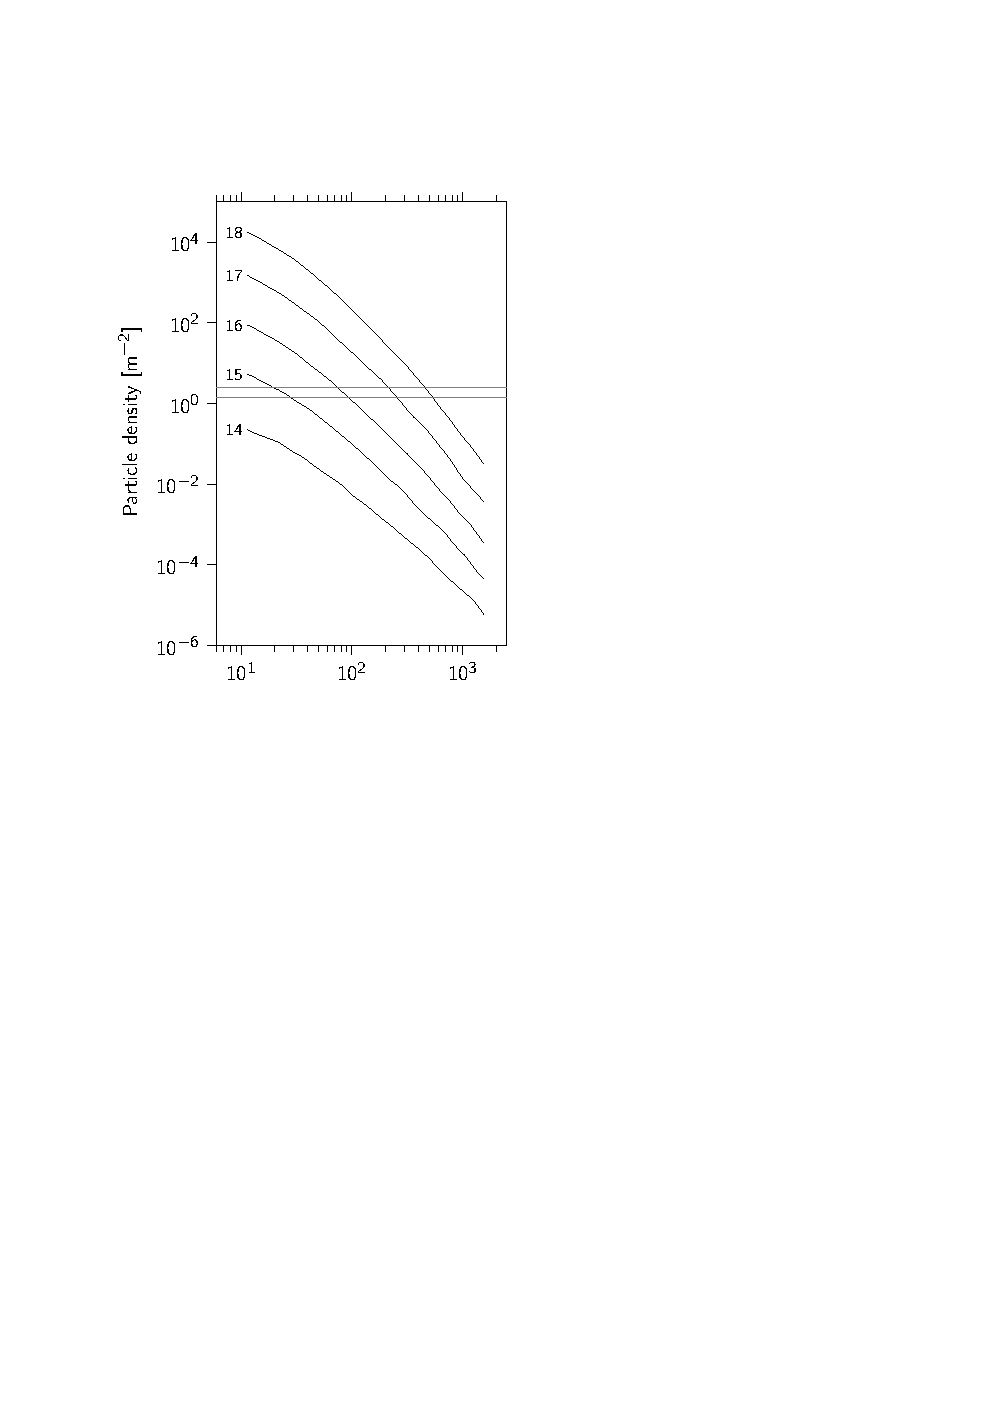
\includegraphics[width=0.6\textwidth]
                    {plots/experiment/ldf_energies}
    \caption{LDF for E = \SIrange{e14}{e20}{\eV} showers (e + mu). This gives the limits of detecting showers, depending on core distance and detector size. (do not show horizontal lines)}
    \label{fig:ldf_energies}
\end{figure}

% What do we want to determine for each air shower; time of arrival, direction of the shower axis, position of the core, and energy of the primary.
% Which properties of the shower need to be measured to determine this
By detecting the arrival time of particles from the same shower at various locations the shower front is sampled. This allows for the reconstruction of the shower. Using the arrival times the direction of the shower can be reconstructed. Using the density the core position and energy can be obtained. These reconstructions are not independent, knowledge about the core position improves direction reconstruction, and vice-versa shower axis direction makes the estimation of expected particle densities more accurate.

% What are the possibilities of identifying a source
The experiment will be based in the Netherlands, with possible extensions to other countries. From the Netherlands the Northern sky is observed. This provides a similar field of view to the TA experiment, which is at latitude \SI{39.3}{\degree}, while \nikhef is at \SI{52.3}{\degree}. The visible skymap, assuming a zenith acceptance of \SI{60}{\degree}, in equatorial coordinates is shown in \cref{fig:visible_sky_map}. The anisotropy measurement of cosmic rays at very high energies is difficult to achieve. The Auger and TA experiments have only a handful of detections above \SI{e20}{\eV}. Measurement of the isotropy at lower energies is also important.

\begin{figure}
    \centering
    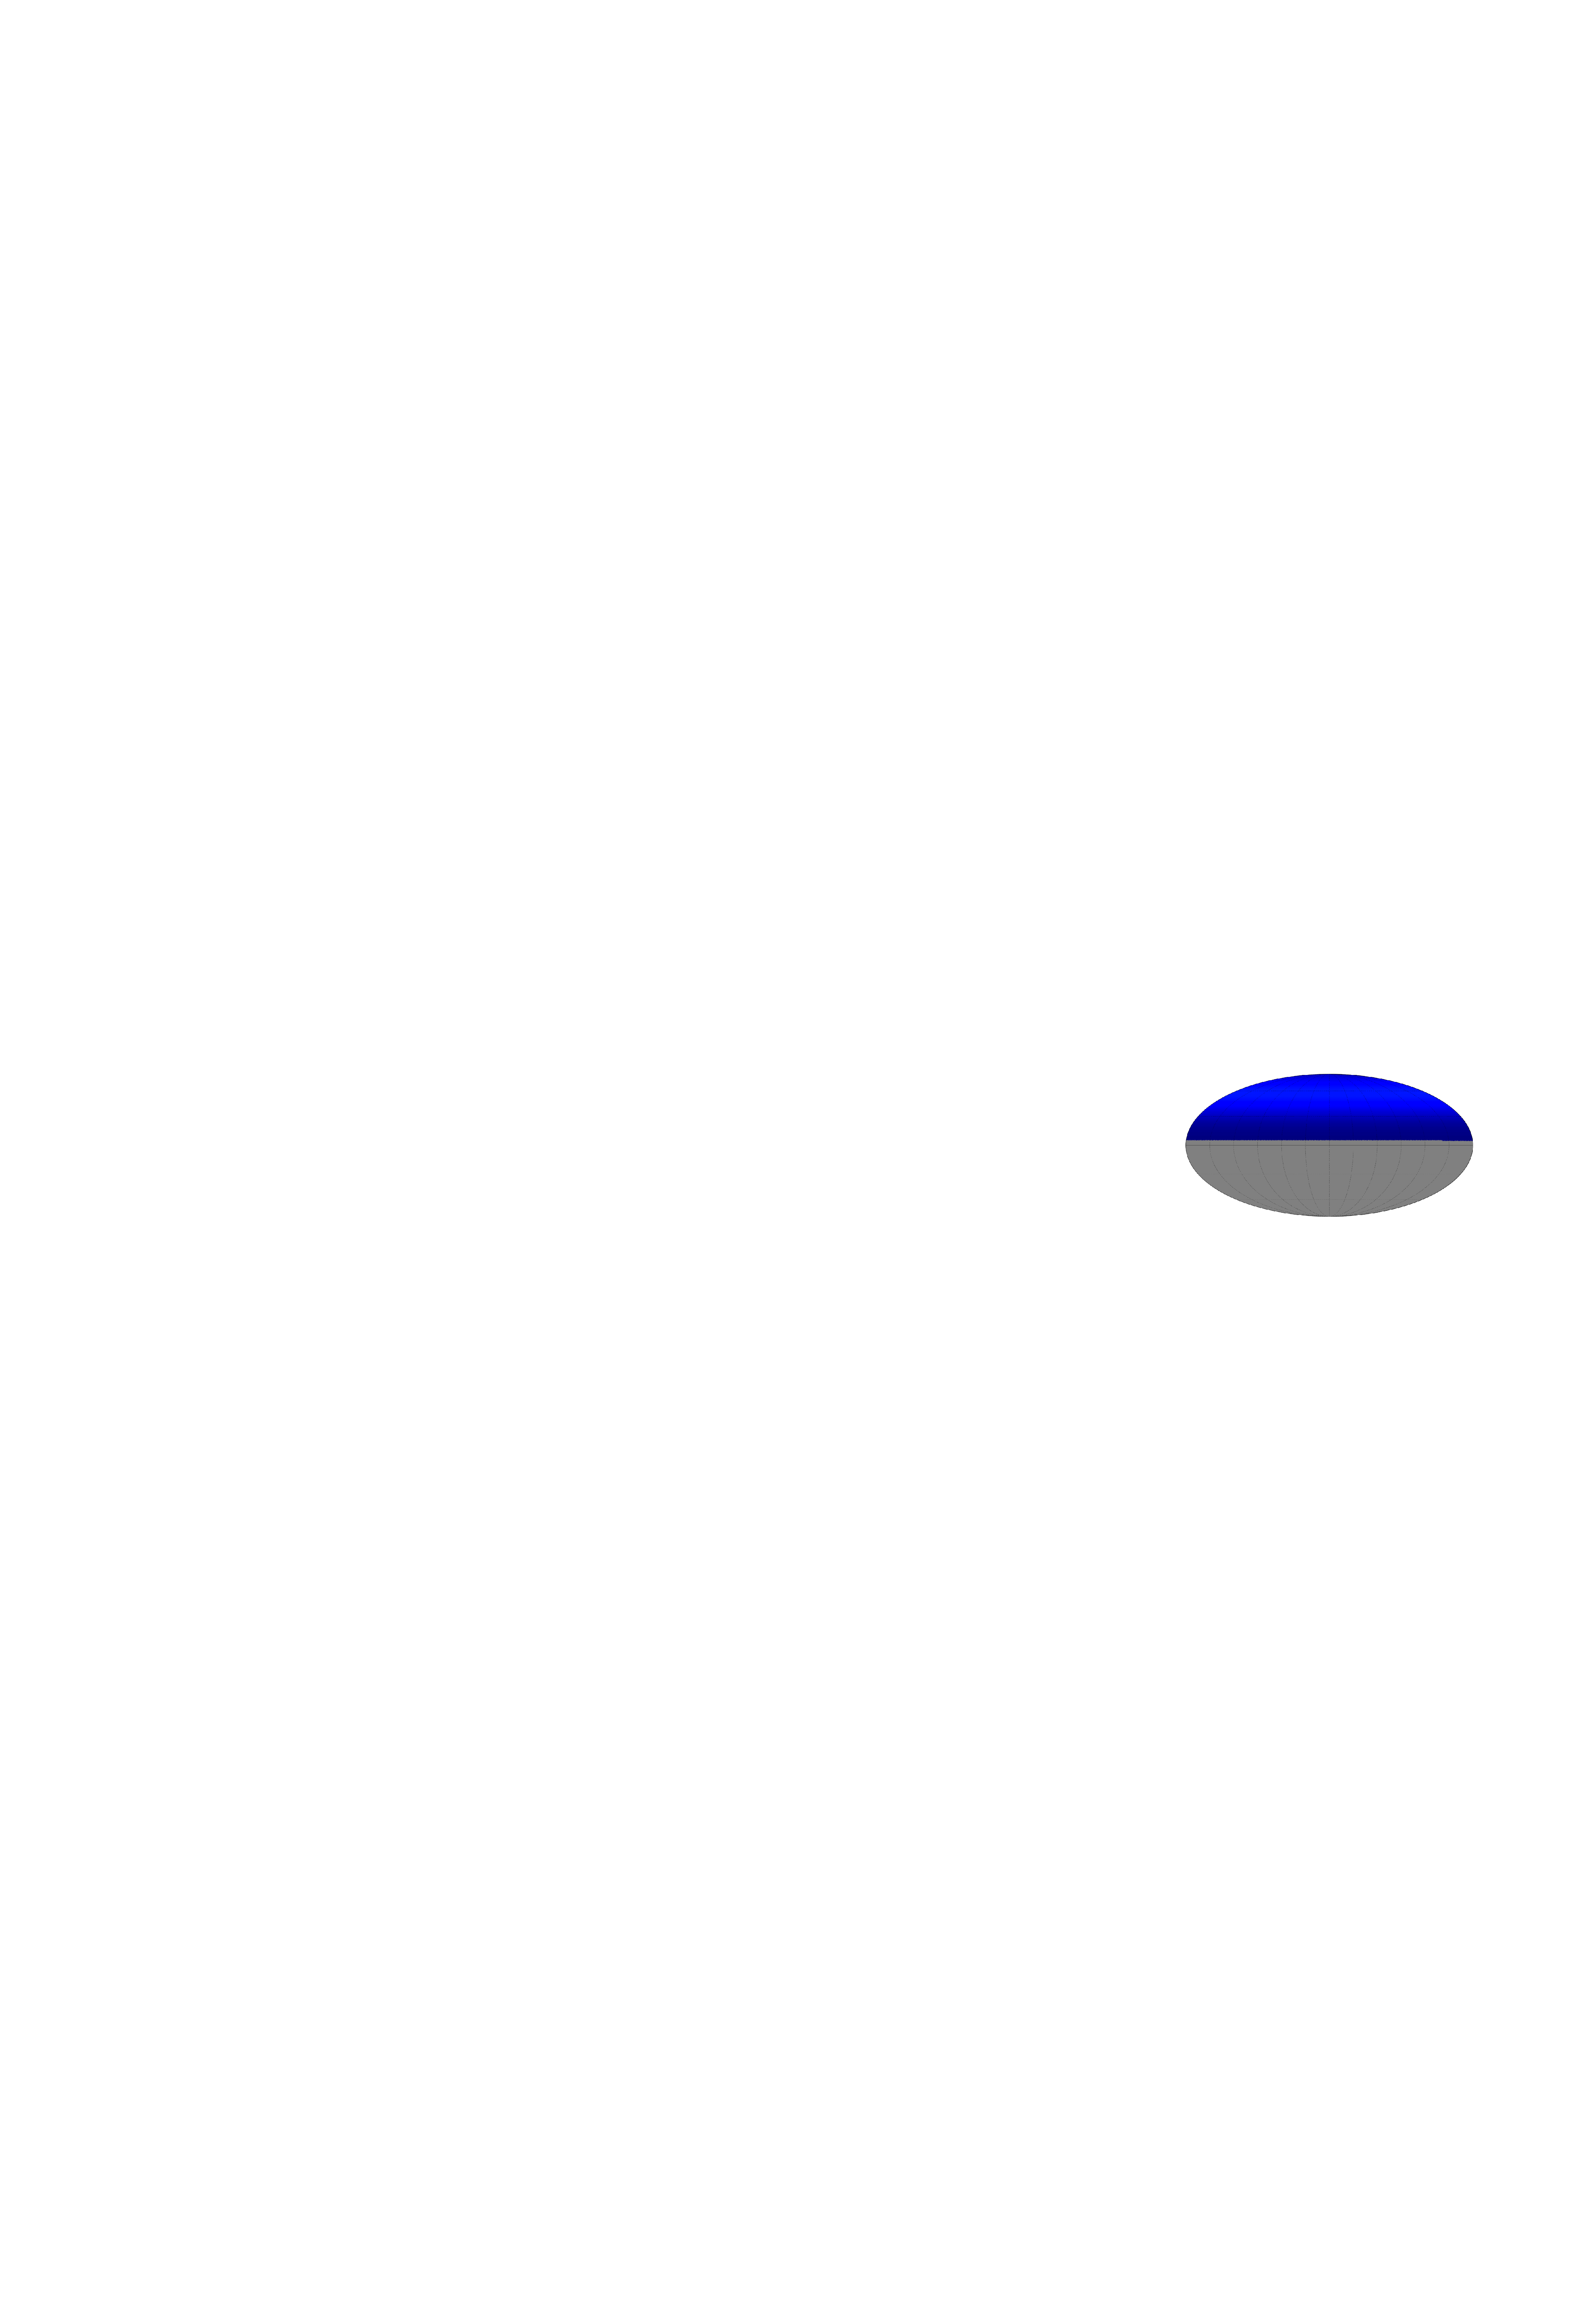
\includegraphics[width=0.6\textwidth]
                    {plots/experiment/visible_sky_map}
    \caption{Equatorial sky map (mollweide) highlighting part of universe which is above the horizon in the Netherlands. Similar field of view to TA/KASCADE.}
    \label{fig:visible_sky_map}
\end{figure}


\section{Design for detection}

% Detector the particles in the shower front, not the fluorescence/Cherenkov. For several reasons; particle detectors are much cheaper, provides higher uptime. Also detect extensive air showers during day time, moon nights, and with other sources of light pollution.
In \cref{sec:other_observables} methods other than particles detectors for the observation of air showers were mentioned. These will not be considered, as these methods are much more expensive and have lower duty cycles. For experiments such as TA and Auger they do provide excellent independent calibration of the surface particle detectors and extra information about the shower This experiment will use particle detectors for the detection of cosmic rays.

% What properties/observables of the air shower particles need to be measured.
%  - Arrival time of the particles (leptons) and their number.
%  - Accurate arrival time is needed for direction (using shower front shape).
%  - Accurate particle count is needed for energy/core (using lateral density).
As stated before the arrival time of particles and number of particles in a detector can be used to reconstruct the shower. The accuracy with which this needs to be measured depend on the properties of the shower and detectors. For increasing detector distance the required arrival time accuracy to achieve the same direction reconstruction accuracy becomes less. With increasing core distance the particle density decreases, while the rise time of the shower front increases. This makes it more likely that the few particles that are detected are further delayed from the causal front.

Also important to consider is the likelihood of actually detecting a shower. For a given particle density ($\rho$) the probability of detecting a certain number ($k$) of particles in a detector with a certain area ($A$) is given by the Poisson distribution,

\begin{equation}
    P_k(\lambda) = \frac{\lambda^k \mathrm{e}^{-\lambda}}{k!} \ ,
\end{equation}

where $\lambda$ is the expected number of particles, i.e. $\lambda = \rho A$. This assumes the detectors are \SI{100}{\percent} efficient at detecting charged particles. The important probability is the probability of not detecting any particle given a particle density $P_0(\lambda) = \mathrm{e}^{-\lambda}$. Which gives the probability of detecting at least one particle via

\begin{equation}
    P_p(\lambda) = 1-P_0(\lambda) \ .
\end{equation}

% Each particle detector will have a background from low energy showers, such showers are very abundant, but only few particles (mainly muons) reach ground level.
Not each detected particle will be desired. A big component of the background comes from low energy showers (\SI{<e14}{\eV}) which produce only a couple muons at ground level. Such low energy cosmic rays are very abbundant. Instead of resulting in an instantaneous high density of particles these showers produce a random background of particles. These showers produce few particles to effectively detect in multiple detectors. In \cref{fig:particle_density} the total particle flux at various atmospheric depths is shown. At ground level the muon flux dominates. Showers of \SI{e13}{\eV} produce an approximately equal number of muons and electrons on ground, below this muons dominate. The high muon flux relative to electrons is dominated by showers below \SI{e13}{\eV}.

\begin{figure}
    \centering
    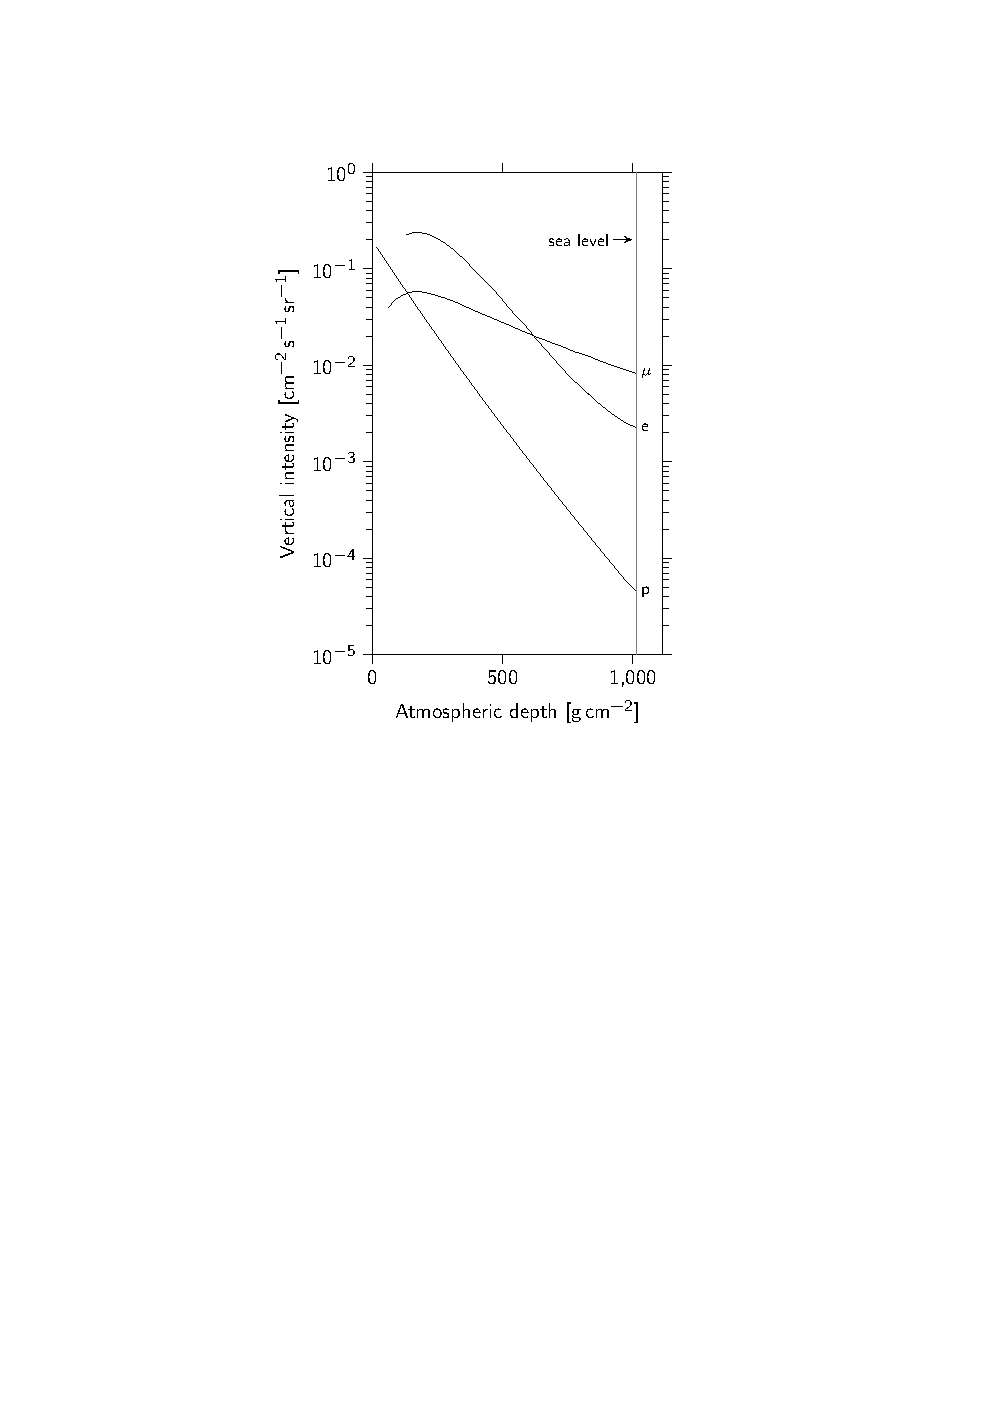
\includegraphics[width=0.6\textwidth]
                    {plots/experiment/particle_density}
    \caption{Particle flux composition as function of atmospheric depth, to show the flux of particles at ground level, todo: filter for only particles with 'enough' energy (like Grupen fig7.10)}
    \label{fig:particle_density}
\end{figure}

% How to filter the background away by using a coincidence trigger. Two (or more) simultaneous, unrelated, detections in separated detectors is unlikely.
By using the fact that the particles from energetic showers are more correlated in time those showers can be distinguished from the background by looking for time-correlated particles. This might be possible with a single detector which looks for short bursts of many particles. However, this does not provide data for reconstruction, since the arrival time and density is only known at one position. Using multiple detectors which need to have a time-correlated detection is more sensitive to lower particle densities and provide data for reconstruction. Using two detectors to disgtinguish the particles from the background by requiring at least one particle in each detector makes the probability detection $P_p^2(\lambda)$, assuming the particle density is equal at both detectors. The size of and distance between the detectors will determine the lower energy limit.

% Why are for reconstruction multiple detection points needed.
To be able to fully reconstruct the direction of an air shower at least three detection points are required. Having two detection points with arrival times provides one constraint on the shower axis, but a plane of possible axes remain, a third point constrains the shower axis. This can either be achieved by a single station with three or more detectors (short distances), or by combining detections from multiple stations (larger distances). Using a 3-detector station the probability of detecting at least one particle in each is given by $P_p^3(\lambda)$. If the station had even more detectors but still required at least 3 in coincidence the probability of detection becomes

\begin{equation}
    P_{min=3}(\lambda) = \sum_{k=3}^{n} \left(^n_k\right) P_p^k P_0^{n-k} \ ,
\end{equation}

where n is the total number of detectors.

% Depending on size of coincidence window how much background remains. Reconstruction should identify bad/accidental events.
Consider the 2-detector setup again in which both need to detect a particle within a short time window to make certain both are from the same shower. The rate of muons at ground level is about \SI{400}{\Pmump\per\meter\squared\per\second}. Most should have entirely uncorrelated arrival times, but since the distribution is random some might arrive simultaneously. The expected rate of coincidences in case all muons have random arrival times is given by

\begin{equation}
    R_{\mathrm{background}} = 2 \tau A^2 f^2 \ ,
\end{equation}

where $\tau$ is the time window, $A$ the detector area, and $f$ the flux. The time window should be at least the distance between the two detectors divided by the light speed. That should be the most extreme case for a shower to arrive horizontally in line with the detectors. Longer time differences are possible due to different transport time in the detector and the rise time and curvature of the shower front.

- Where should the detectors be placed (relative to each other)
  - For low energy (\SIrange{e14}{e15}{\eV}) showers the detectors need to be closely spaced (\SI{10}{\meter}) otherwise the density in the detectors becomes to low to effectively detect them.
  - For high energy (\SIrange{e18}{e20}{\eV}) showers the detectors need to be placed further apart (\SI{>500}{\meter}) otherwise the area covered by the detectors is to small and only few high energy showers will be detected.

% The detectors need to be reliable to prevent continuous maintenance tasks, and to last the length of the experiment, MoU expects ~5 years.
Ideally the detectors operate without maintenance. But the components might have finite lifetimes or require recalibration after some time. If many detectors require frequent service and maintenance this will cost time that could otherwise be spent on data anlysis. Basically the costs of the experiment go up. Using tried-and-tests components that have been shown to be reliable for long periods are prefered.

% Cost effective detectors so high-schools can participate in the project
Making detectors larger makes them more likely to detect particles. The downside is that the detector becomes less easy to handle, more expensive, efficiency uniformity may worsen, and saturation might occur sooner. A good balance needs to be determined.

% The detector needs to be safe to handle by students
% Detectors need to be durable so they can survive the typical Dutch weather
The experiment is meant to be accessible for high schools, the detectors need to be fairly easy to handle. If the detectors would be placed inside schools the roof material might affect the detections. In order to have enough space to place the detectors the most obvious location would be on the roof. If the detectors are outside proper protection from weather effects need to be considered.


\section{Detector}

% Using scintillators with PMTs provide good particle detection efficiency, \SI{100}{\percent} of energetic leptons are detected, also some gammas are seen.
The detector consists of two main components which perform the detection. The scintillator, which emits light when charged particles pass through it, and the Photomultiplier tube (\pmt) which converts the scintillation photons into an electric signal.

% Scintillator size and material
Scintillators have been selected as detection material. This is a relatively cheap material with high reliability and excellent efficiency. The scintillator is a sheet of \SI[product-units=power]{100 x 50 x 2}{\centi\meter} made from BC-408 \cite{bc408}. The BC-408 material has good timing properties and light output for charged particles.

% PMT size and type
The chosen photomultiplier tube \cite{et:pmt} is a compact \SI{29}{\milli\meter} (effectively \SI{25}{\milli\meter}) diameter and \SI{~11}{\centi\meter} long \pmt. The quantum efficiency of the biakali photocathode is \SI{28}{\percent} [check this value] for the wavelength of the scintillation light. The \pmts have a number of dynodes The \pmts are very efficient at amplifying faint light pulses to measureable electric signals. Several brands and types of \pmts have been used. At first \pmts (including power supply) were sourced from Electron Tubes, ET Enterprises and Sens-Tech, later new \pmts were constructed using Hamamatsu tubes with a \nikhef power supply. The \nikhef power supply was also compatible with the previously used tubes, and can serve to replace a broken power supply.

Besides these the detector construction consists of several other components. An isosceles triangle light guide [measurements] made from polymethylmethacrylate (PMMA). The light guide is glued to the scintillator using Optical Cement (\cite{bc600}). A little adapter piece (same material as light guide) is attached to the square end of the triangle with Optical Cement and the round window of the \pmt with optical tape [type?]. This construction is wrapped in thin, \SI{30}{\micro\meter}, aluminium foil with patches of thicker, ??, aluminium foil at the corners of the scintillator, to prevent the sharp edges from piercing the thin foil. This is then wrapped in thick, ??, light tight black pond foil to keep light out and protect the aluminium foil from outside influences.

% Material is mostly 'off the shelf'. Construction/assembly can be performed by students.
All components are readily available from suppliers and not specifically designed for \hisparc.

\begin{figure}
    \centering
    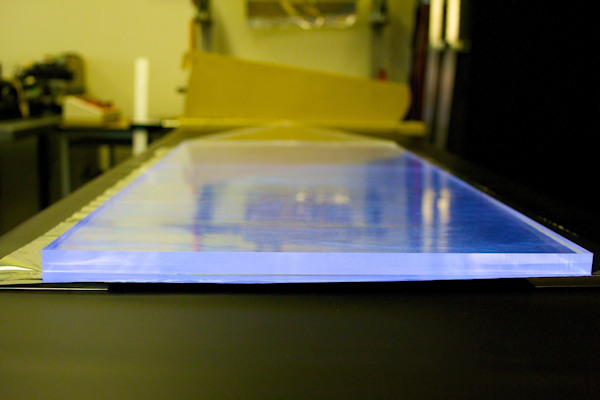
\includegraphics[width=0.6\textwidth]
                    {plots/experiment/ADL_115651.jpg}
    \caption{Show a schematic/photo of detector, indicating the various components.}
    \label{fig:schematic_detector}
\end{figure}

% Detector is protected by skibox from weather and is secured in place by weights.
The final detector dimensions (approximately \SI[product-units=power]{200 x 50 x 3}{\centi\meter} fit well in the chosen detector casing, namely, roof boxes (in Dutch generally referred to as `ski box'). These can be securely fastened and are designed to withstand all kinds of weather. Access to the detector for maintenance is also easy. Also with maintenance in mind, the optical tape with which the \pmt is attached allows it to be easily replaced.


\subsection{The scintillator}

% How Scintillator works
Charge particles loose energy in the scintillator in interactions with the base of the scintillator, polyvinyltoluene. Ionization is the main source of energy loss for energetic charged particles (electrons, muons). The base will emit photons which are rapidly absorbed by the fluor of the scinatillator, anthracene. The fluor then emits light at a lower wavelength, to which the scintillator is more transparent. Some of this light will reach the \pmt.

% Most shower muons/electrons are minimum ionizing particles (mips) and have similar energy loss in the detectors, given by Bethe-Bloch (spread on energy loss given by Landau).
The mean amount of energy deposited by the particle going through the detector is described by the Bethe-Bloch formula. This gives the amount of energy lost by the particles per \si{\gram\centi\meter\squared} of the material it passes through. However, the interactions in which the particles loose energy is a statistical process, the energy loss is not a fixed number but a distribution, the Landau distribution. The ionization energy loss for

The scintillator is \SI{2}{\centi\meter} thick, however, many particles have a longer path through it because they travel at an angle. This increases the expected mean energy loss. The path can also be shorter if the particle passes through one of the sides of the scintillator, but due to the large area of the detector relative to its thickness the chance of that happening is low.

% Signal transport efficiency not uniform for the detector due to geometry.
The light emitted along the path of the particle is transmitted in random directions. Depending on the angle at which the emitted photons hit the outer edges of the scintillator there is a chance that they will be reflected back or leave the scintillator. The entire detector is wrapped in aluminium foil to attempt to reflect those photons back into the scintillator. To detect the photons they need to hit the photocathode of the \pmt. To get to the \pmt they need to pass from the scintillator through a layer of optical glue, the light guide, another layer of optical glue, a small piece of light guide, and a layer of optical tape to reach the \pmt. During this most photons will be reflected a number of times. For \SI{1}{\mip} approximately 30000 photons [check.] are emitted, the fraction that reach the \pmt depend on the location in the scintillator where the particles are emitted. A 2D Monte Carlo simulation of the detector [cite Jos Steijger] predicts the transmission efficiency from locations in the scintillator to the \pmt. The resulting transmission efficiency distribution is shown in [fig of tranmission efficiency].


\subsubsection{Gammas in the scintillator}

Energetic photons can also deposit energy in the scintillator due to Compton scattering and pair creation. However, the cross sections for these interactions is very low. A \SI{1}{\MeV} photon  has a mean free path greater than \SI{10}{\centi\meter}, which increases further for higher energy photons, see fig [By Jos/Tom]. Despite the low detection chance, the large number of photons in an air shower makes them statistically relevant.


\subsection{\pmt}

% How PMT works
The photomultiplier tube has a front window with a photocathode. When this is hit by a photon an electron can be knocked free, due to the photoelectric effect. The electron is then pulled along electric field lines which direct it to a dynode. The electron will cause multiple electrons to be emitted from the dynode, these electrons are then pulled to the next dynode, which has a higher positive potential. The electrons impacting this dynode will each cause the release of more electrons, which are accelerated towards the next dynode. At the end the electrons fall on the anode which is connected to the readout. The used PMTs have 11? (SensTech) and 12? (Hamamatsu) dynodes, this number affects the gain of the PMT. If each electron causes \num{3} electrons to be released from a dynode then every electron falling on the first dynode will result in $3^{n_{\mathrm{dynodes}}}$ electrons at the anode.

% Signal strength is used for particle density, need to be able to distinguish between different number.
Both the scintillator and \pmt can handle multiple particles simultaneously and will produce correspondingly higher signal output. The integrated signal strength should be the sum of two individual particles. Given the signal distribution for single particles given by the Landau distribution combined with the transport efficiency one particle will in some (how often?) produce a signal equal or larger than the most probable signal strength of two particles.

- Fast ADC readout of the PMT provides accurate timing.


\begin{figure}
    \centering
    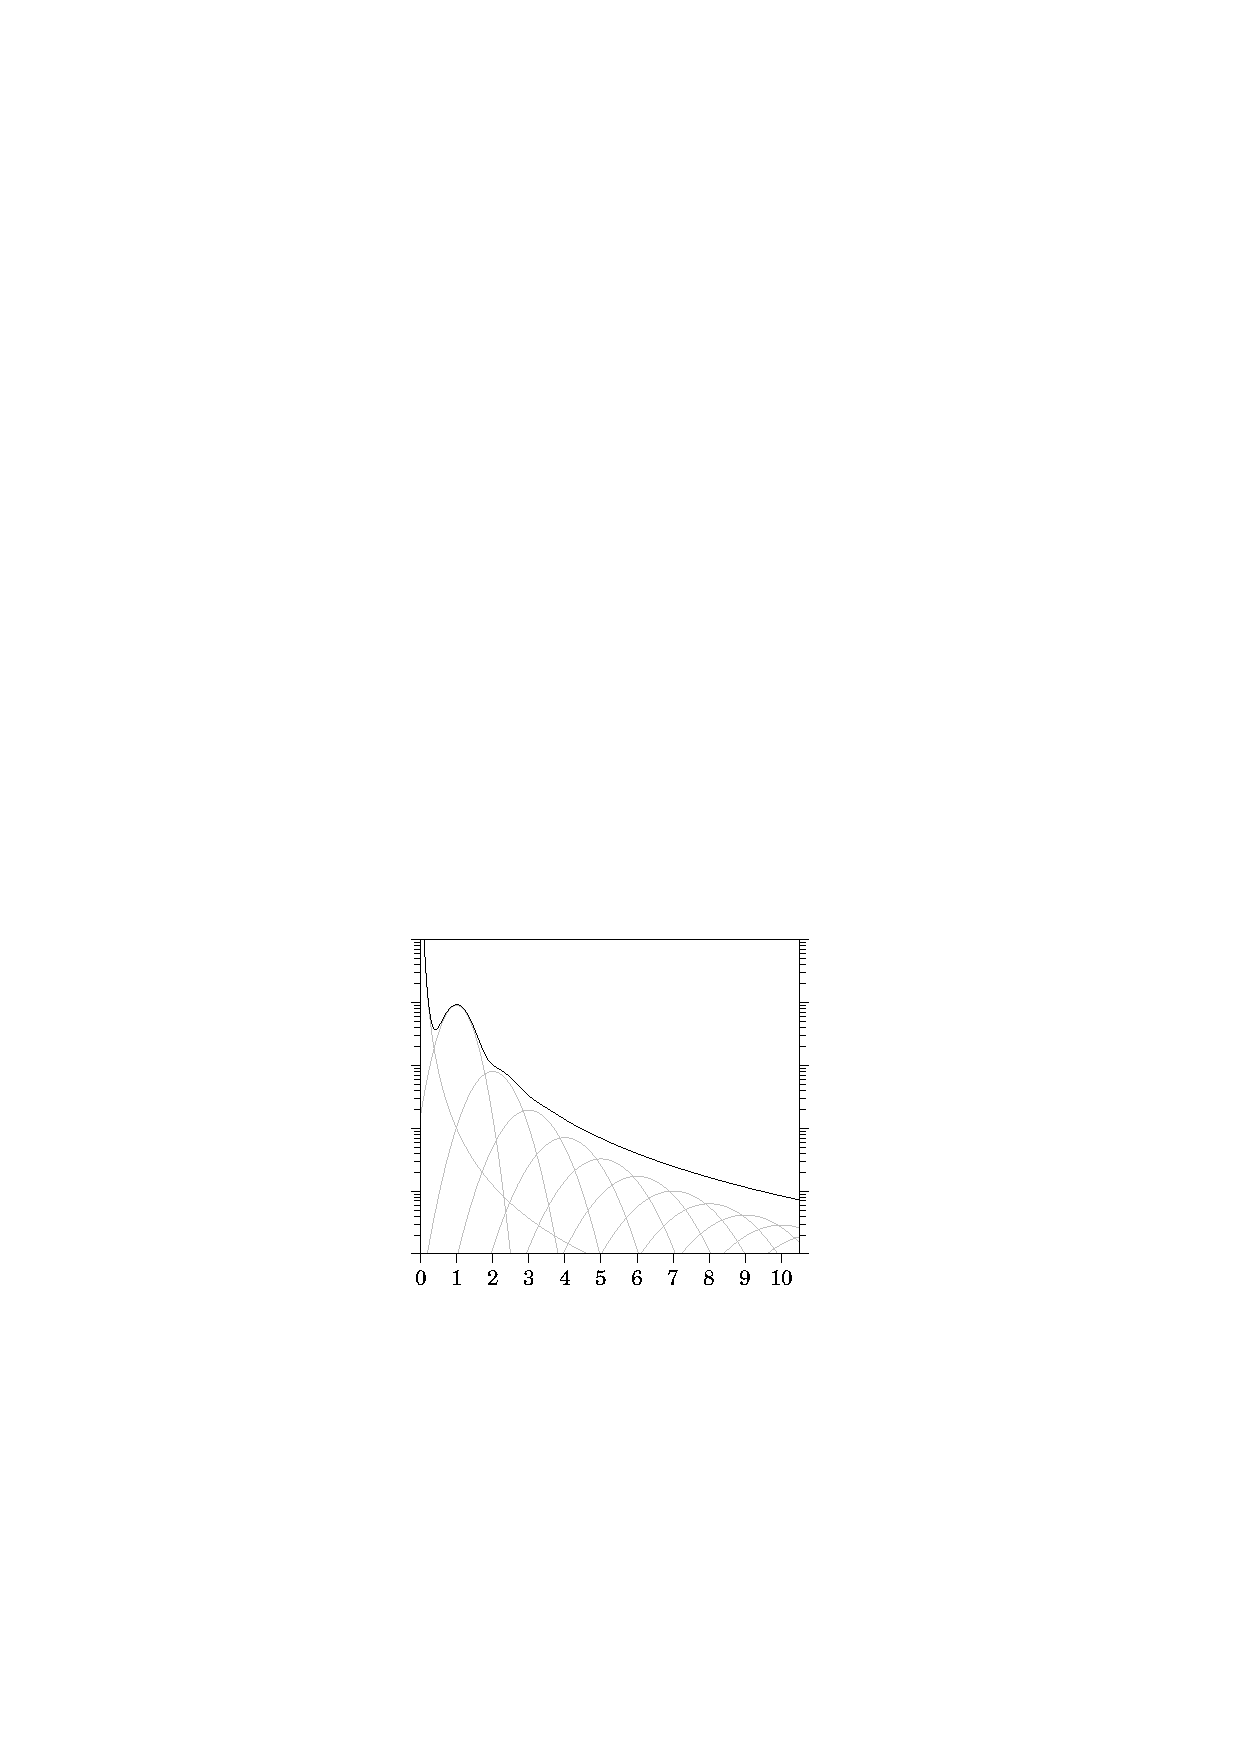
\includegraphics[width=0.6\textwidth]
                    {plots/experiment/ph_histogram_contrib}
    \caption{Overlap between pulse integral contributions from multiple mips in one event, the with of each contribution is due to Landau distribution and transport efficiency.}
    \label{fig:ph_histogram_contrib}
\end{figure}


\begin{figure}
    \centering
    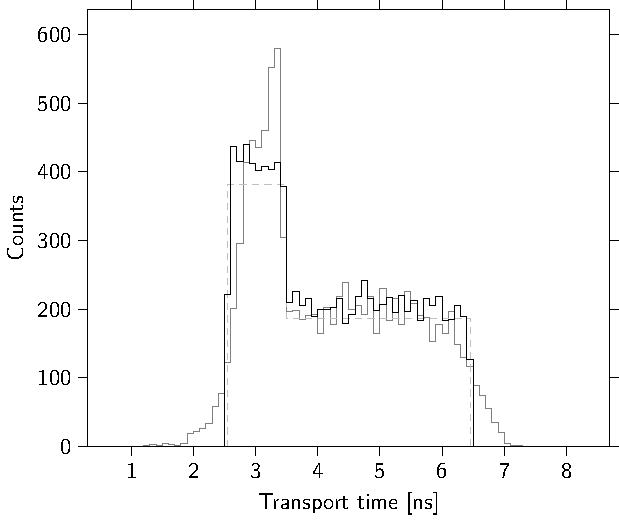
\includegraphics[width=0.6\textwidth]
                    {plots/experiment/transport_time}
    \caption{Transport time distribution for the detector. The scintillation light has to reach the PMT from the point of impact, the travel time depends on the impact location, this is the distribution for the entire detector.}
    \label{fig:transport_time}
\end{figure}


\section{Station}

- Impractical to connect detectors over long distances for online/realtime triggering.

- Multiple detector readout with ADCs, use the good timing for coincidence time trigger.

- An efficient trigger can be made for a certain (and higher) particle density.

- For (low energy) shower detection a station has multiple detectors close together and contains the trigger logic.

- For high energy showers the density still needs to be high enough in a station for a trigger, this limits maximum core distance for showers.

- Using more than two detectors in a station increases detection efficiency.

- More than two detectors have the possibility of direction reconstruction.

- Explain simple direction reconstruction with 3 detection points (flat/curved shower).

- Trigger efficiency as function of core distance and shower energy, for the different triggers (2 in 2-detector, any 2 in 4-detector, and any 3 in 4-detector for reconstructable).

- Standard layouts created to encourage uniformity, these are also chosen for good shower acceptance, reconstruction accuracy of station events, and practicality for the locations.

- Shower core/energy determination impractical with single station.

\subsection{Weather station}


- Optional weather station to provide local weather data.

- May not be required at each station, can use freely available KNMI data. However, in some cases closest KNMI station is far away.


\begin{figure}
    \centering
    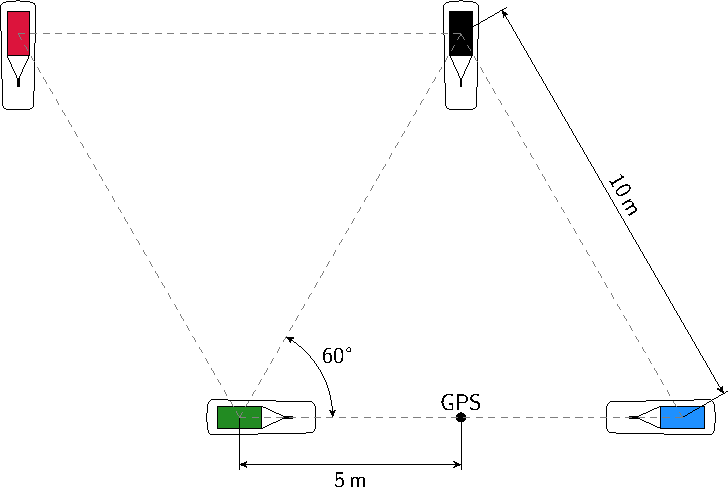
\includegraphics[width=0.4\textwidth]
                    {plots/experiment/4_detector_diamond}
    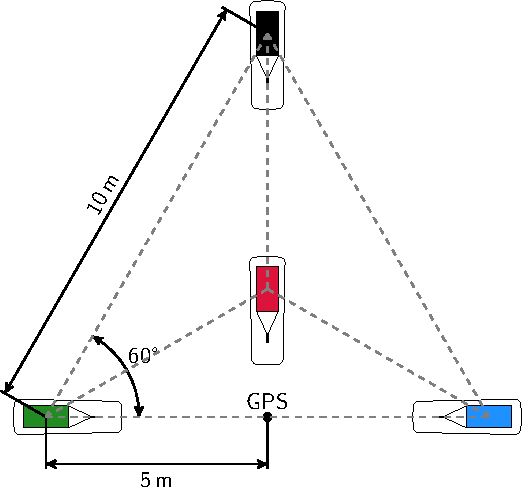
\includegraphics[width=0.4\textwidth]
                    {plots/experiment/4_detector_star}
    \caption{4-detector station layouts. 4-detector stations are typically placed in the diamond or star formation. Both contain multiple triangles between sets of 3 detectors.}
    \label{fig:4_detector_star}
\end{figure}


\begin{figure}
    \centering
    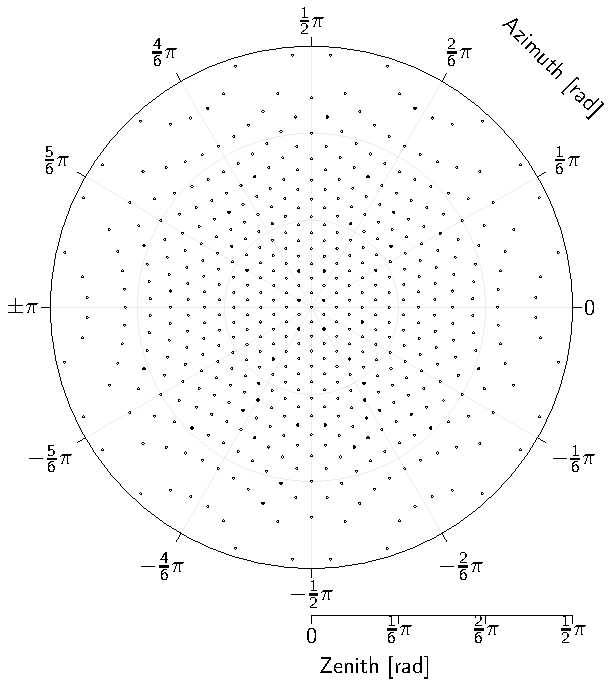
\includegraphics[width=0.6\textwidth]
                    {plots/experiment/discrete_directions}
    \caption{Both 4-detector layouts result in the following distribution of possible shower directions given \SI{2.5}{\ns} arrival time sampling in the detectors. For the diamond layout more points can be made by more combinations, i.e. more possible solutions. Approximately \SI{5}{\degree} between adjacent points near Zenith.}
    \label{fig:discrete_directions}
\end{figure}


\begin{figure}
    \centering
    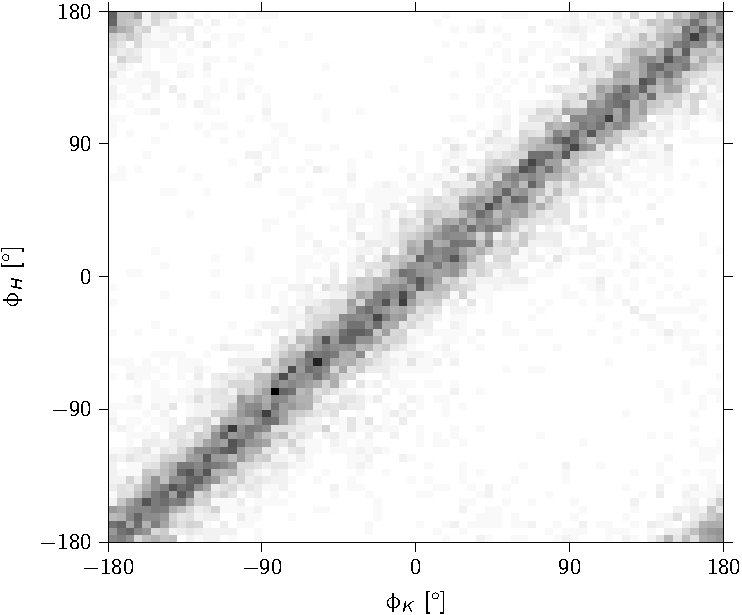
\includegraphics[width=0.6\textwidth]
                    {plots/experiment/azimuth_kascade_minn1}
    \caption{Test station at KASCADE was used to verify the performance of a single station. The direction agreement between simultaneously detected events is shown.}
    \label{fig:azimuth_kascade_minn1}
\end{figure}

\begin{figure}
    \centering
    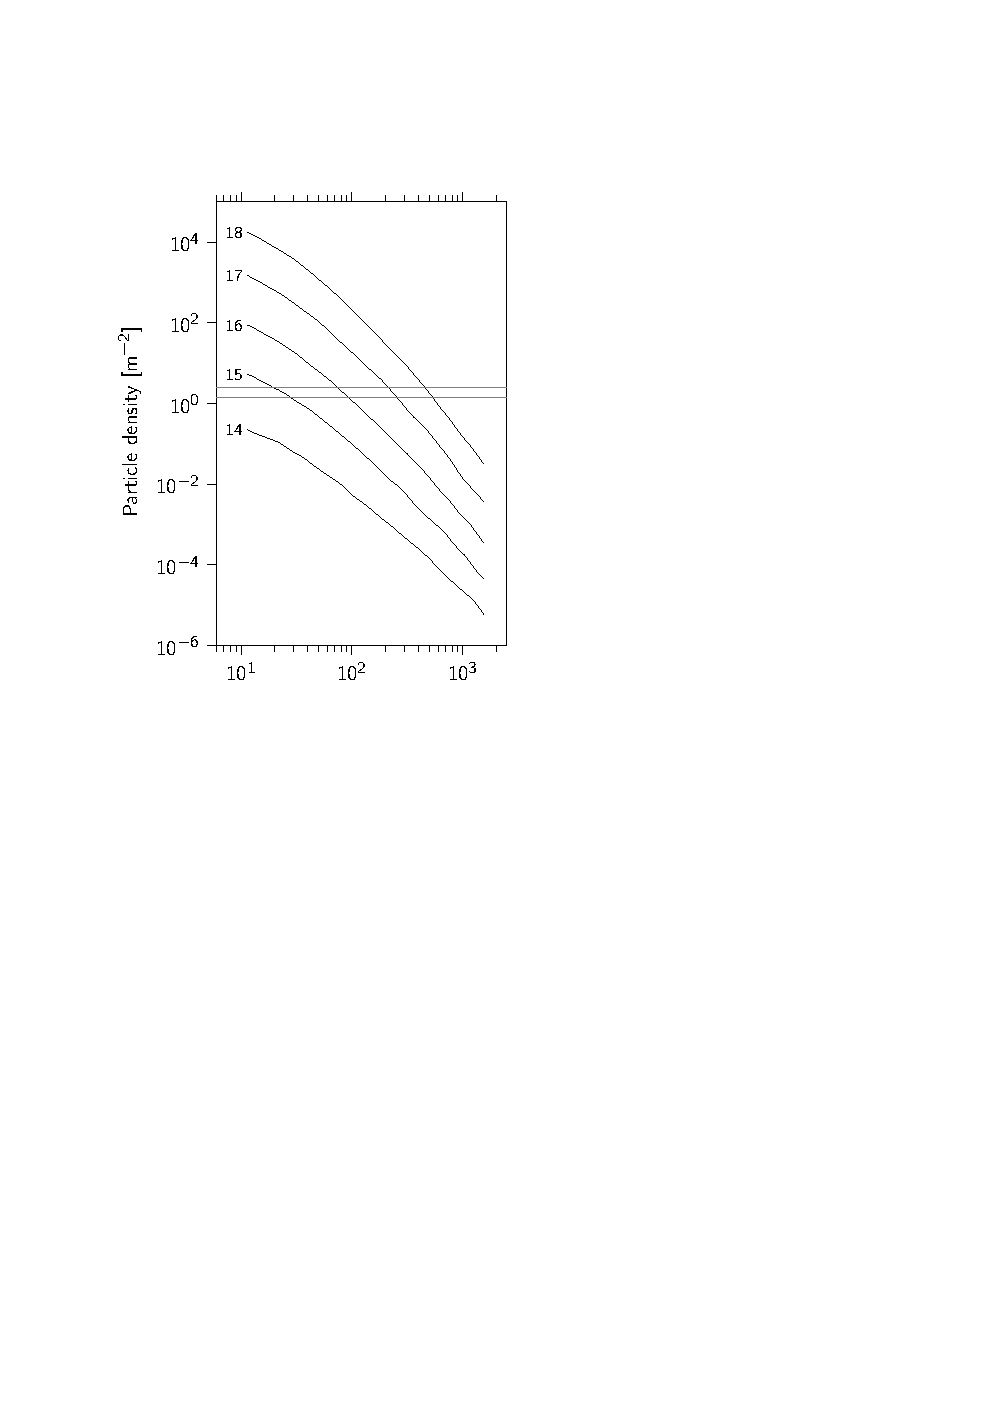
\includegraphics[width=0.6\textwidth]
                    {plots/experiment/ldf_energies}
    \caption{Trigger efficiency E = \SIrange{e14}{e20}{\eV} showers, add horizontal lines for 2 in 2-detector, any 2 in 4-detector, and any 3 in 4-detector (\SI{50}{\percent} efficient, perhaps also \SI{~100}{\percent} efficiency lines).}
    \label{fig:ldf_energies2}
\end{figure}


\begin{figure}
    \centering
    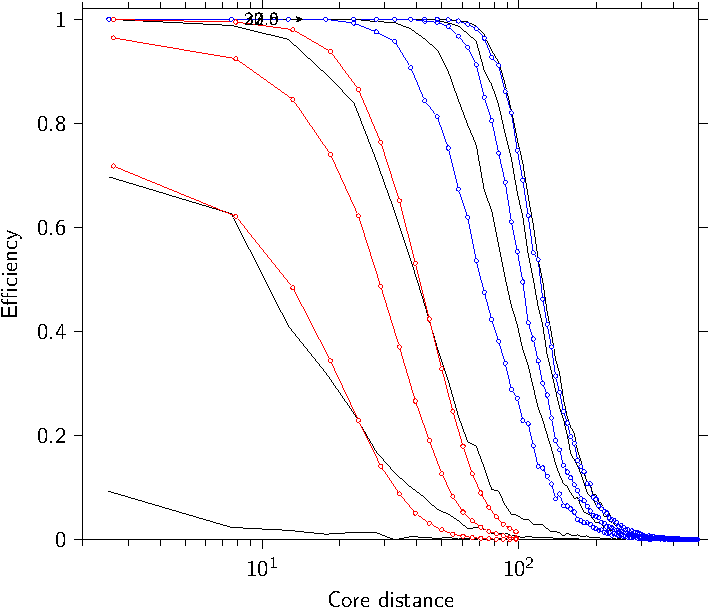
\includegraphics[width=0.6\textwidth]
                    {plots/experiment/efficiency_two_16}
    \caption{Detection (trigger) efficiency as a function of core distance for showers of different primary energy (and zenith).}
    \label{fig:efficiency_two_16}
\end{figure}


\begin{figure}
    \centering
    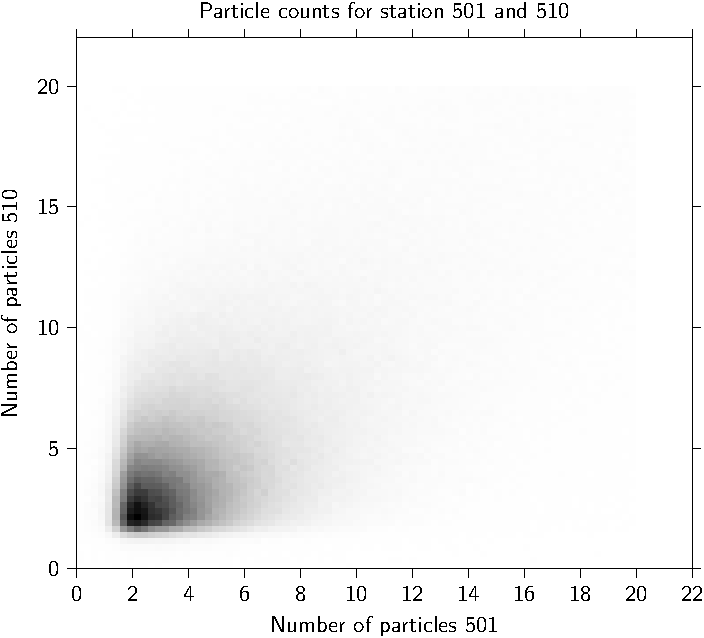
\includegraphics[width=0.6\textwidth]
                    {plots/experiment/n_501_510_sum}
    \caption{(place holder figure showing different data) Test station at KASCADE used to verify the particle density measurement of a single detector and full station, compared to the KASCADE predicted particle density.}
    \label{fig:n_501_510_sum}
\end{figure}



\section{Network}


- Each station submits data/triggered events to central datastore

- Use offline analysis to find station events detecting the same shower.
    - This requires good absolute timing at the stations.
    - Use GPS at stations for both positioning of the stations (\SI{~1}{\meter}) and absolute timing (\SI{~5}{\ns}).

- Current station locations, explain why the stations are in those locations. Due to those being the locations of high schools..

- Stations closer than \SI{2e3}{\meter} are likely to detect the same shower.

- Similar direction reconstruction algorithm as used for single station.

- At large core distances the curvature of the shower front should be taken into account.

- For a large event should arrival times in each detector be used or station average density and average/first arrival time?

\begin{figure}
    \centering
    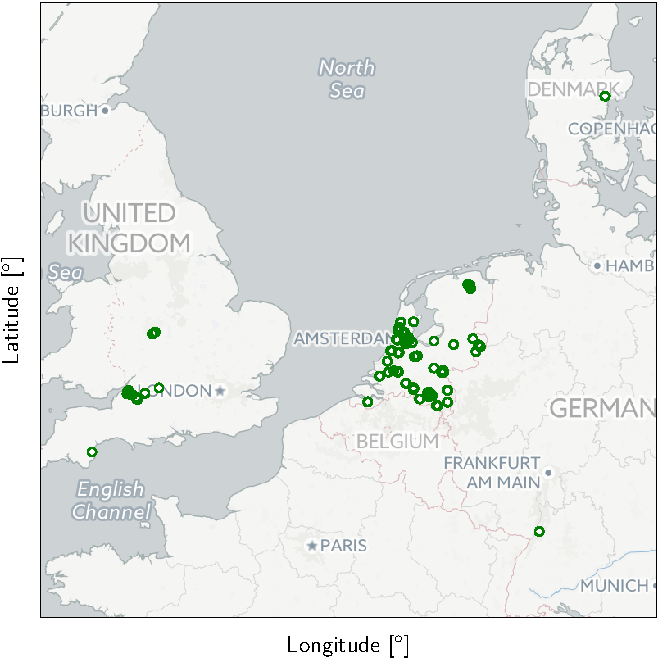
\includegraphics[width=0.6\textwidth]
                    {plots/experiment/network}
    \caption{Location of HiSPARC stations in Netherlands, United Kingdom, and Denmark.}
    \label{fig:network}
\end{figure}


\begin{figure}
    \centering
    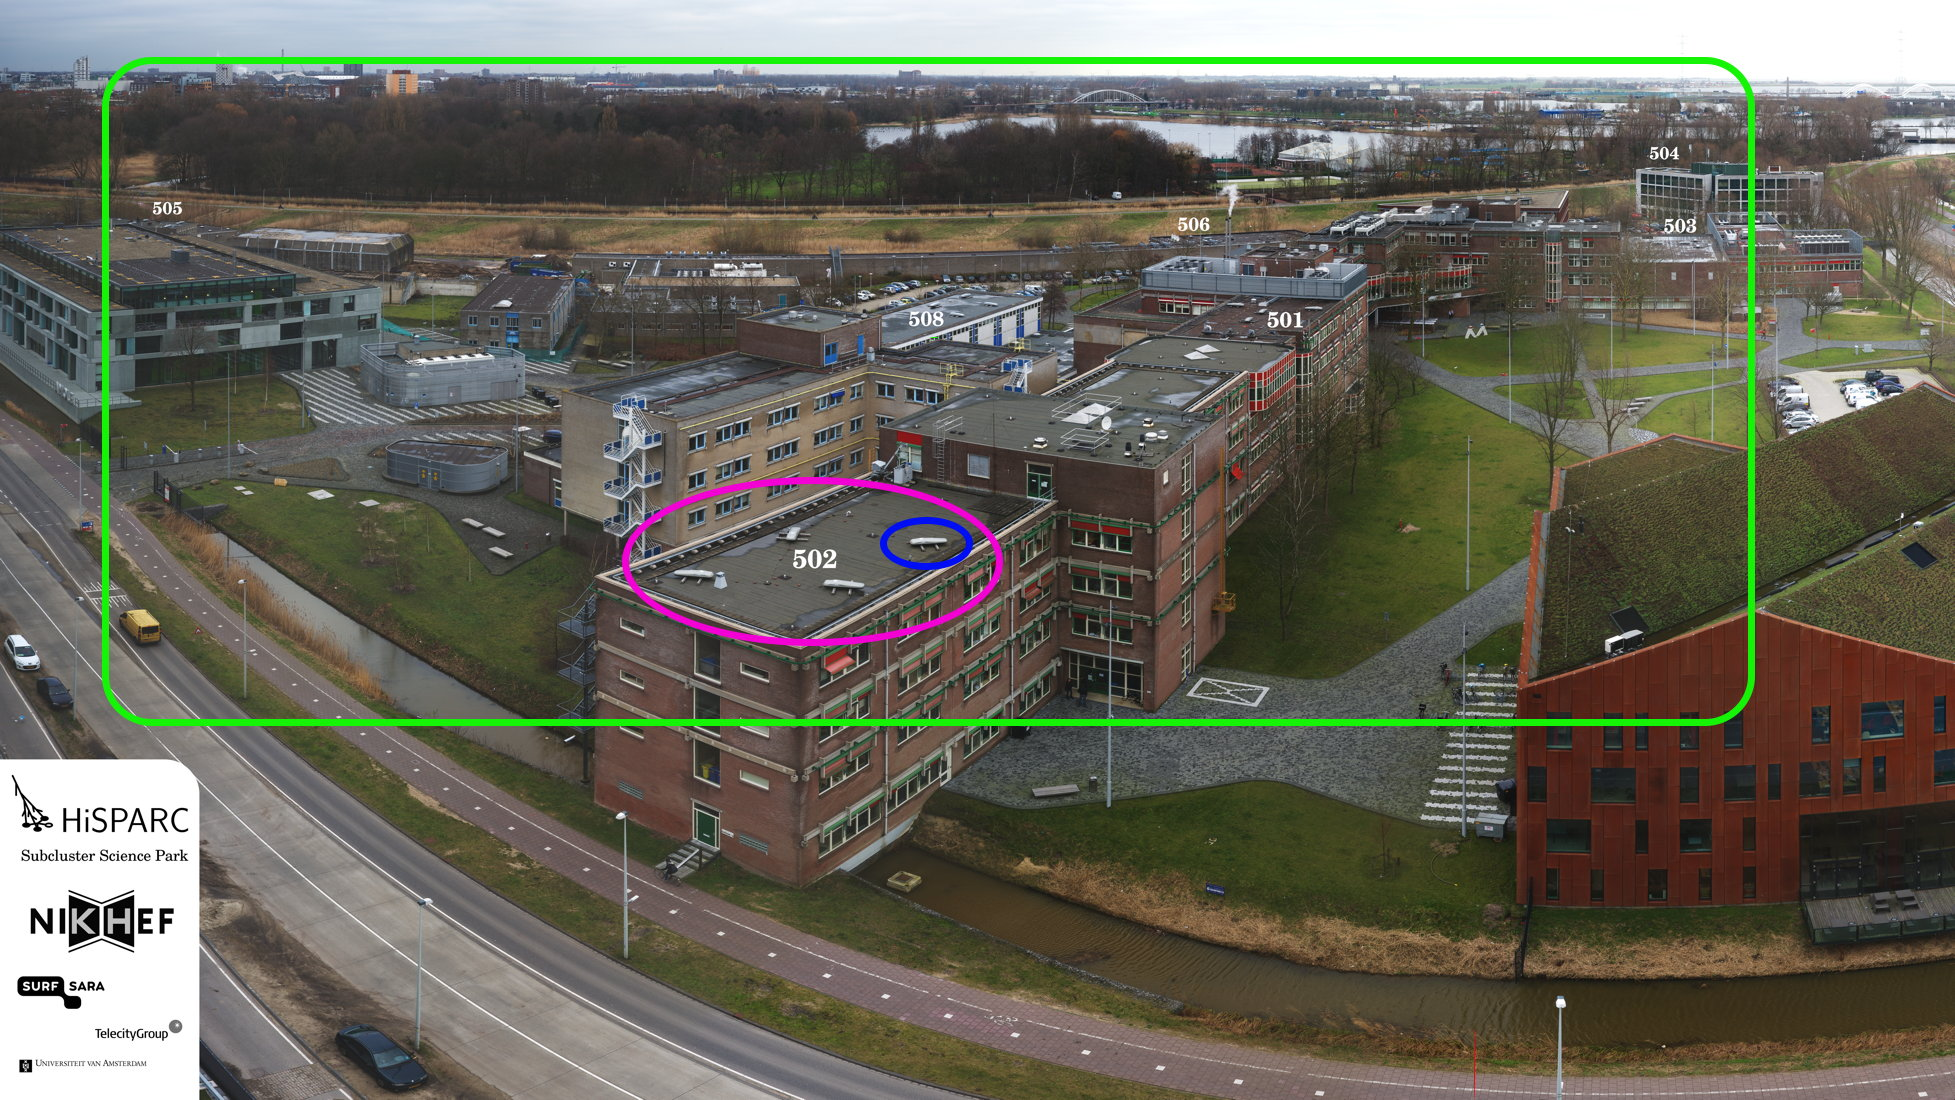
\includegraphics[width=0.6\textwidth]
                    {plots/experiment/ADL_151373_151429_layers.jpg}
    \caption{Show what a collection of stations look like. Highlight a single detector, a station, and a collection of stations.}
    \label{fig:ADL_151373_151429_layers}
\end{figure}


\begin{figure}
    \centering
    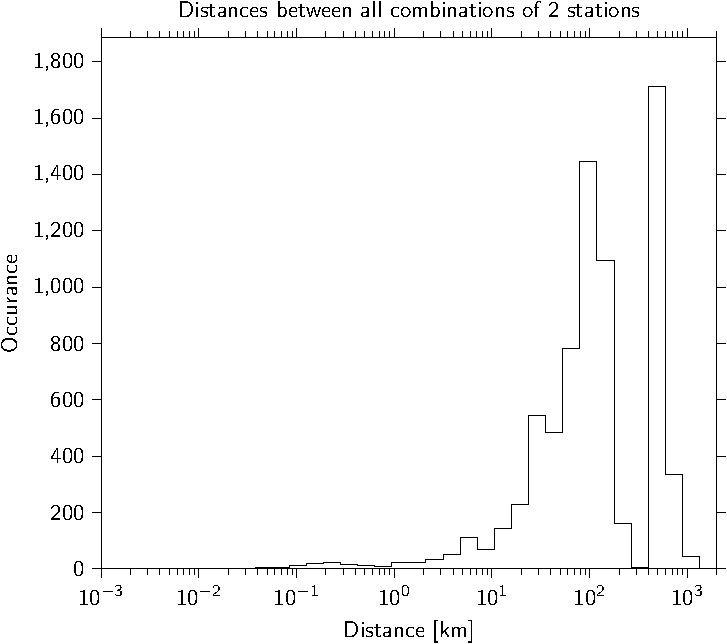
\includegraphics[width=0.6\textwidth]
                    {plots/experiment/network_station_distances}
    \caption{Distribution of distances between all possible pairs of stations in the entire HiSPARC network.}
    \label{fig:network_station_distances}
\end{figure}


\begin{figure}
    \centering
    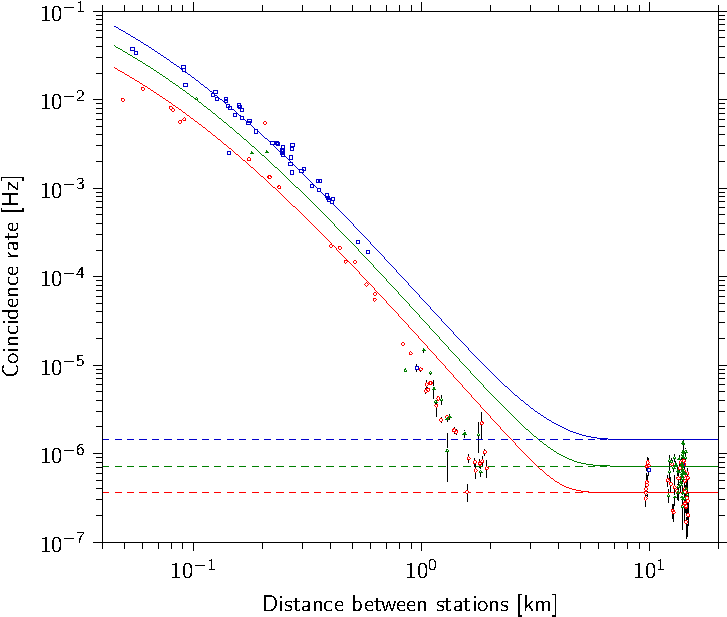
\includegraphics[width=0.6\textwidth]
                    {plots/experiment/distance_v_coincidence_rate}
    \caption{Coincidence rate between stations as a function of distance. At increasing distances the contributions from increasingly larger/energetic showers dominate. The background rate is also shown. Real events may still be distinguished from background}
    \label{fig:distance_v_coincidence_rate}
\end{figure}


\begin{figure}
    \centering
    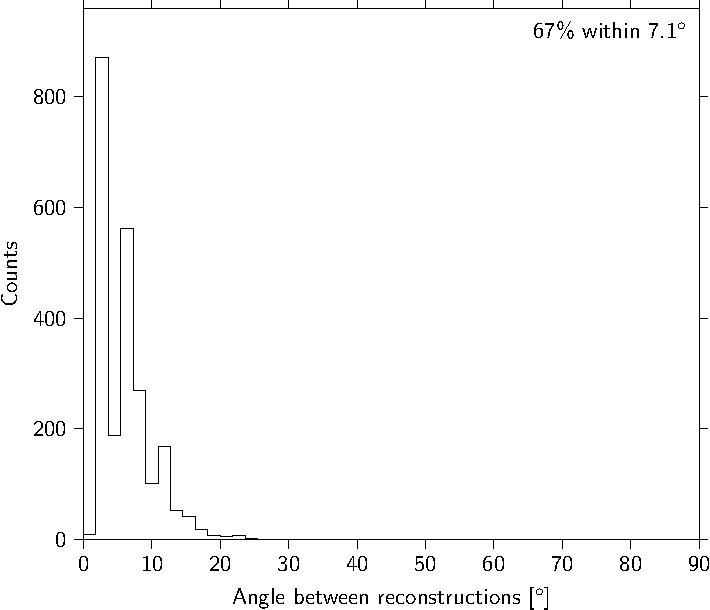
\includegraphics[width=0.6\textwidth]
                    {plots/experiment/angle_between_501_minn16_510}
    \caption{(placeholder plot, not data mentioned in caption) Distance between reconstructions when using average/first arrival time, versus simulation input. Using separate detectors should hold more information, but the reconstruction algorithm should be aware (using curved or flat reconstruction?)}
    \label{fig:angle_between_501_minn16_510}
\end{figure}


\begin{figure}
    \centering
    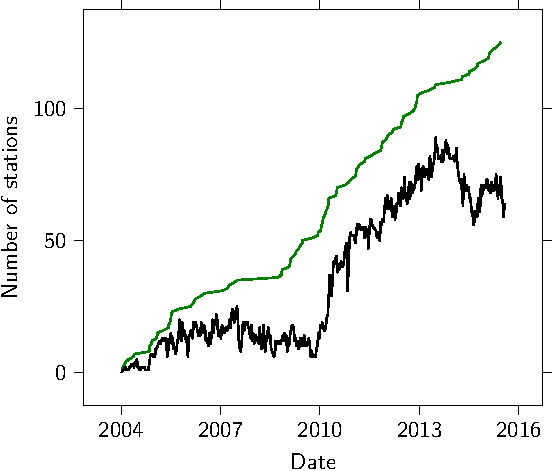
\includegraphics[width=0.6\textwidth]
                    {plots/experiment/active_stations}
    \caption{Cumulative number of stations with at least an hour of good data and the number of active stations per day.}
    \label{fig:active_stations}
\end{figure}

\begin{figure}
    \centering
    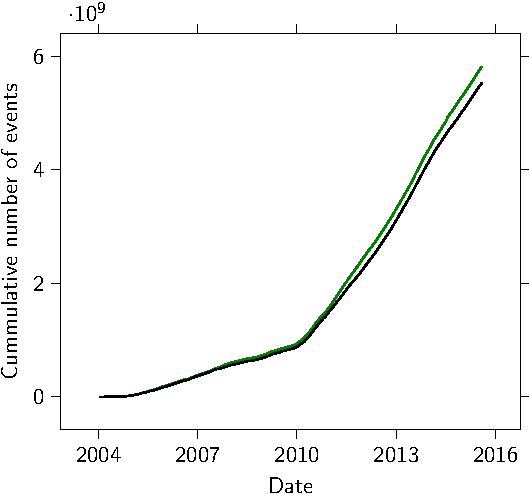
\includegraphics[width=0.6\textwidth]
                    {plots/experiment/luminosity_network}
    \caption{Cumulative number of events by all stations, the lower line contains only events when the stations were working properly.}
    \label{fig:luminosity_network}
\end{figure}

